\paragraph{Projected geometry and reference samples.}
Figure~\ref{fig:fermat-section} uses a curved section of the Fermat quintic,
a Calabi--Yau hypersurface \citep{hendi2024invariant}. The section is
projected to $\R^3$ and approximated by 325 Gaussian tubes with equal masses
and covariance $0.035^2I_3$. The projection and coordinate-grid law are given
in Appendix~\ref{app:fermat-construction}. This example has three observed
coordinates, unlike the density heights in Figures~\ref{fig:elvis-example}d
and~\ref{fig:volcano}a.

\begin{figure}[t]
\centering
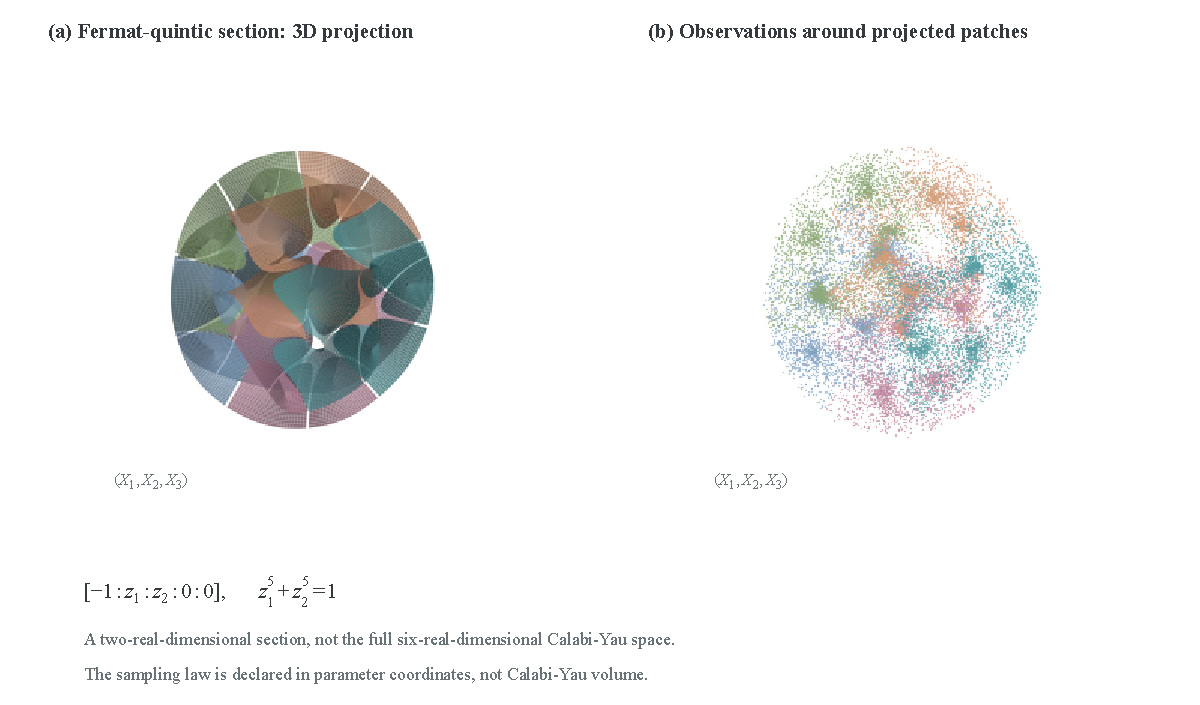
\includegraphics[width=0.97\linewidth,clip]{figures/fermat_section.pdf}
\caption{A projected Fermat-quintic section and an SFD around it. Left:
the geometric patches, colored by root index. Right: 18,000 observations
from 325 Gaussian tubes. Both panels use three spatial coordinates.}
\label{fig:fermat-section}
\end{figure}

Figure~\ref{fig:reference-histograms} complements these declared-geometry
examples with empirical views of Gaussian, skew-mixture and banana-transform
reference samples. Joint and marginal histograms expose different aspects
of the same sample shape. Each display uses 500 stored training observations;
the fitted-method comparisons begin in Section~\ref{sec:experiments}.
Appendix~\ref{app:visual-examples} records the construction details for
Figures~\ref{fig:elvis-example}--\ref{fig:reference-histograms}.

\begin{figure}[t]
\centering
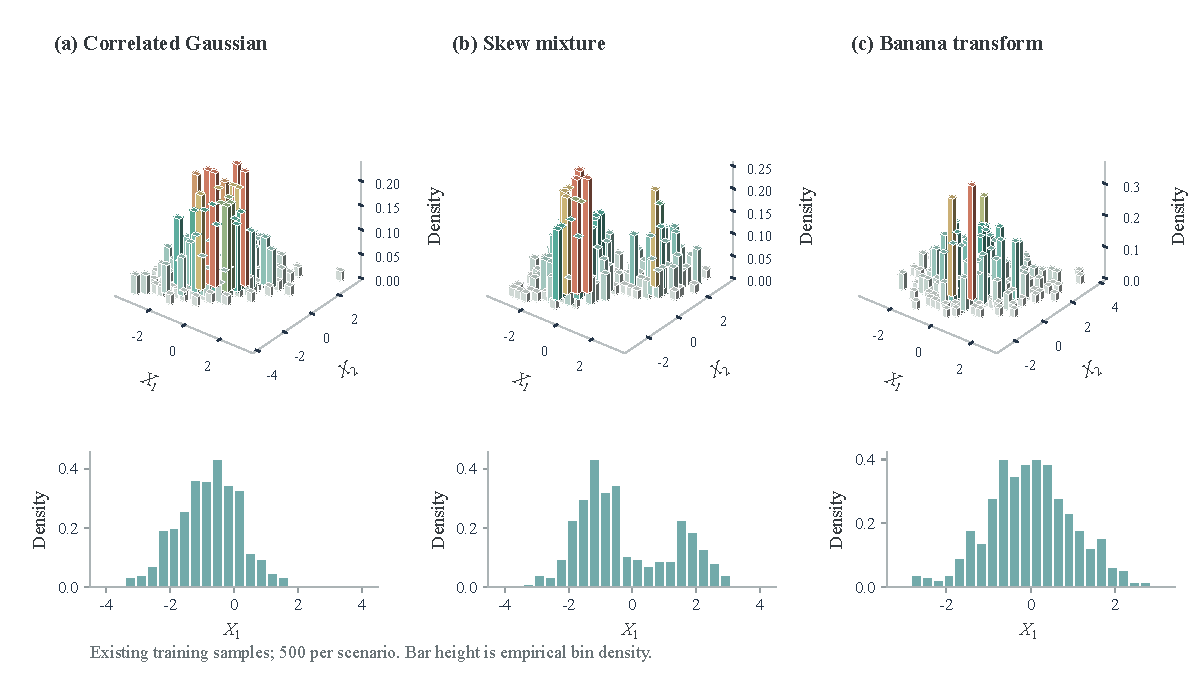
\includegraphics[width=0.97\linewidth,clip]{figures/reference_histograms.pdf}
\caption{Reference-sample histograms for a correlated Gaussian, skew mixture
and banana transform. Top: $24\times24$ bin densities in the first two
coordinates. Bottom: first-coordinate marginals. Each scenario uses all
500 training draws.}
\label{fig:reference-histograms}
\end{figure}

\paragraph{Density surfaces.}
Figure~\ref{fig:density-examples} shows four specified bivariate laws,
including a Doraemon-style face. These are density surfaces over two
coordinates, not three-dimensional observation models. Appendix~
\ref{app:visual-examples} records the display transformation.

\begin{figure}[t]
\centering
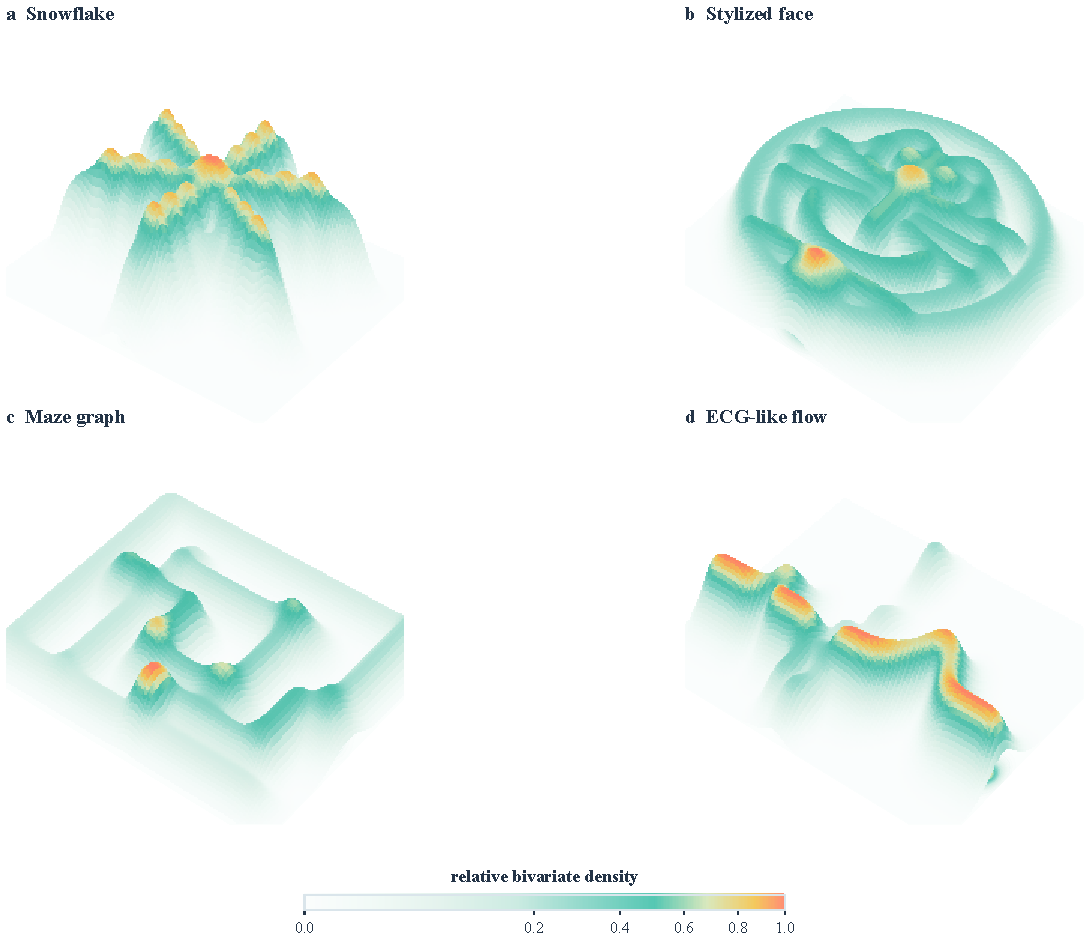
\includegraphics[width=0.94\linewidth,clip]{figures/specified_density_surfaces.pdf}
\caption{Specified snowflake, Doraemon-style face, maze and ECG-like
densities. Height and color use a separate nonlinear relative scale in each
panel, revealing shape rather than comparing absolute density. Curves
contribute Gaussian tubes; localized peaks are Gaussian blobs.}
\label{fig:density-examples}
\end{figure}
